% IOP Publishing format (iopjournal.cls), converted 2026-11-03 from the REVTeX version preserved in
% review/pre_iop_2026-11-03/. All numerical tables are generated from results/revised.
\documentclass[12pt]{iopjournal}
\setlength{\headheight}{15pt}
\usepackage[T1]{fontenc}
\usepackage{amsmath,amssymb,placeins}
\usepackage[numbers,sort&compress]{natbib}
\hypersetup{pdftitle={Finite-cycle sensitivity and phase-resolved amplification in effective loop quantum Bianchi IX cosmology},pdfauthor={Muhammad Ramadhan}}
\newcommand{\Lam}{\Lambda}
% primitive input, so that \hline may follow the generated rows inside a tabular
\makeatletter\newcommand{\tabrows}[1]{\@@input generated/#1.tex }\makeatother
\newcommand{\KBounce}{0.15}
\newcommand{\KCycle}{3.81}
\newcommand{\KLongB}{3.95}
\newcommand{\KLongR}{3.81}
\newcommand{\ABounce}{0.14}
\newcommand{\ACycle}{3.94}
\newcommand{\ALongB}{3.81}
\newcommand{\ALongR}{3.78}

\begin{document}

\articletype{Paper}

\title{Finite-cycle sensitivity and phase-resolved amplification in effective loop quantum Bianchi IX cosmology}

\author{Muhammad Ramadhan}

\affil{Department of Informatics Engineering, Universitas Hasanuddin, Gowa, Indonesia}

\email{ramadhaanm@gmail.com}

\keywords{loop quantum cosmology, Bianchi IX, Mixmaster universe, quantum bounce, sensitivity to initial conditions, deterministic chaos}

\begin{abstract}
Effective loop quantum cosmology replaces the singular contraction of the Bianchi IX universe with
bounce--recollapse cycles. We quantify the sensitivity to initial data of two effective quantizations, based on extrinsic-curvature (K) and connection (A) holonomies, using outcome labels and trajectory separations sampled at volume extrema and at specified phase markers. Sampling at these events removes the dependence on the time parametrization of the integration, although the finite-time distances still depend on an explicit choice of phase-space coordinates and norm. The directional scale factors are monitored along each trajectory, the integration stops at the first sub-Planckian crossing or numerical failure, and physical exits are reported separately from unresolved integrations. For an initial rescaling $\Lam=20$, the median logarithmic amplification from the first to the second
recollapse is $\KCycle$ and $\ACycle$ decades in the K and A models, respectively, for pairs passing
linearity and noise controls. The marker-defined bounce window contributes $\KBounce$ and
$\ABounce$ decades. We also report the dependence on the initial scale, the phase thresholds, and stricter axis-length cutoffs, and we examine a six-cycle ensemble in extended precision. These are conditional finite-time
measurements: they provide evidence of strong recurrent sensitivity, but do not establish an
asymptotic fractal basin boundary, a universal mixing rate, or preservation of information in the full
quantum state. The results show that the amplification is concentrated outside the chosen bounce window,
consistent with earlier observations of strong sensitivity near recollapse.
\end{abstract}

\section{Introduction}
The Belinskii--Khalatnikov--Lifshitz (BKL) conjecture motivates a description of the approach to a
generic spacelike singularity by approximately local sequences of Kasner epochs, interrupted by
curvature transitions~\cite{BKL1970}. The homogeneous Bianchi IX, or Mixmaster, universe is an
important prototype~\cite{Misner1969,HeinzleUggla2009,Ringstrom2001,DamourHenneauxNicolai2003}.
Its classical chaotic dynamics can be studied through the uncertainty exponent of outcome
boundaries~\cite{CornishLevin1997}. Time parametrization requires care: numerical Lyapunov exponents
are not invariant under arbitrary changes of clock, although the characterization of chaos is
invariant under transformations satisfying appropriate hypotheses~\cite{Motter2003,MotterSaa2009}.
Comparisons made at geometrically defined events therefore offer a useful complementary diagnostic.

In effective loop quantum cosmology (LQC), a quantum-geometric bounce replaces the singular contraction
in many homogeneous models~\cite{AshtekarWilsonEwing2009,WilsonEwing2010}. In closed Bianchi IX models,
bounces can be followed by classical recollapses. Early studies involving inverse-volume effects
suggested suppression of Mixmaster chaos~\cite{BojowaldDate2004,BojowaldDateHossain2004}, whereas later
work emphasized sensitivity accumulated across repeated classical segments~\cite{WilsonEwing2019}.
Blackmore and Wilson-Ewing numerically found nearby solutions separating especially strongly near
recollapse and comparatively little at the bounce~\cite{BlackmoreWilsonEwing2023}.
This qualitative mechanism is therefore already established, and it motivates the present measurements.

Different quantum treatments need not agree on this question. Deformed-algebra and generalized-uncertainty
approaches~\cite{BarcaGiovannetti2025,SegretoMontani2025}, quantum moments~\cite{Bojowald2024},
Wheeler--DeWitt wave packets~\cite{LoFrancoMontani2026}, and volume polymerization~\cite{MuzammilHusain2025}
modify different parts of the dynamics. We restrict attention to two specified effective holonomy
Hamiltonians without inverse-triad corrections. We do not test the full quantum dynamics or attempt to decide between these models.

Recent work quantified the incomplete development of classical mixing before a Planck-scale
curvature cutoff~\cite{BrizuelaUriaWilsonEwing2026}. This raises a related finite-time question:
how much sensitivity accumulates in the separate portions of a bouncing cycle? Our contribution
is an ensemble measurement based on a common event construction, a comparison of the K and A quantizations,
pathwise validity checks, and explicit numerical and statistical controls. Throughout, we distinguish finite-cycle amplification from claims about asymptotic chaos or information-theoretic mixing.

\section{Effective LQC of Bianchi IX}\label{sec:model}

We consider the diagonal vacuum Bianchi IX metric $ds^2=-N^2dt^2+\sum_ia_i^2\sigma_i^2$, with $\sigma_i$ the
left-invariant one-forms on $S^3$, and use units $G=\hbar=1$. In terms of the densitized-triad variables
$p_1=a_2a_3$, $p_2=a_1a_3$, $p_3=a_1a_2$ and their conjugates $K_i$, $\{K_i,p_j\}=8\pi\delta_{ij}$, the
Hamiltonian constraint with lapse $N=\sqrt q$, $q=p_1p_2p_3$, reads
\begin{align}
  \mathcal C&=-\frac{1}{8\pi}\sum_{i<j}p_ip_jK_iK_j+U,\label{eq:classical}\\
  U&=\frac{1}{32\pi}\Big[\sum_i\Big(\frac{p_jp_k}{p_i}\Big)^2-2\sum_ip_i^2\Big],\nonumber
\end{align}
where $(i,j,k)$ is a cyclic permutation and ${}^3\!R=-16\pi U/q$. We verified equation~\eqref{eq:classical} against the curvature of the Bianchi IX metric computed directly in Euler coordinates (appendix~\ref{app:checks}).

The first effective model, which we call the K quantization, follows
references~\cite{SinghWilsonEwing2014,BlackmoreWilsonEwing2023}. Holonomies of the extrinsic curvature
replace $K_i$ by $\sin\theta_i/(\gamma\bar\mu_i)$, with $\theta_i=\gamma\bar\mu_iK_i$,
$\bar\mu_i=\sqrt{\Delta p_i/(p_jp_k)}$, $\Delta=4\sqrt3\pi\gamma$ and $\gamma=0.2375$, so that
\begin{equation}
  \mathcal C_K=-\frac{q}{8\pi\gamma^2\Delta}\sum_{i<j}\sin\theta_i\sin\theta_j+U .
  \label{eq:K}
\end{equation}

The second model, the A quantization, is Wilson-Ewing's effective constraint~\cite{WilsonEwing2010},
built from holonomies of the Ashtekar--Barbero connection $c_i=\gamma K_i+\Gamma_i(p)$, where $\Gamma_i$
is the spin connection. Because $\Gamma_i=\partial_{p_i}F(p)$ for some $F$, the map $(c,p)\to(K,p)$ is
canonical, and we find that for $\ell_o=1$ Wilson-Ewing's classical constraint coincides \emph{exactly}
with equation~\eqref{eq:classical}. The two quantizations therefore share the same classical limit and
differ only by quantum corrections. Written in the present variables, equation~(4.2) of
reference~\cite{WilsonEwing2010} (with $r_o=2$) reads
\begin{equation}
  \mathcal C_A=-\frac{q}{8\pi\gamma^2\Delta}\sum_{i<j}s_is_j+\frac{1+\gamma^2}{\gamma^2}\,U
  -\frac{1}{8\pi\gamma^2\sqrt\Delta}\sum_k\frac{(p_ip_j)^{3/2}}{\sqrt{p_k}}\,s_k,\label{eq:A}
\end{equation}
with
\[
  s_i=\sin(\theta_i+\phi_i),\qquad
  \phi_1=\frac{\sqrt\Delta\,(a_1^2-a_2^2-a_3^2)}{2a_1a_2a_3}\quad(\text{and cyclic})
\]
where in the last sum of equation~\eqref{eq:A} $(i,j)$ are the two indices different from $k$. Compared
with equation~\eqref{eq:K}, the holonomies are shifted by the spin-connection phases $\phi_i$, a term
linear in $s_k$ appears, and the potential is rescaled; the classical limit of all three modifications
is exactly equation~\eqref{eq:classical}. The spin-connection phases depend on anisotropy as well as on
overall size, so the magnitude of the difference between the two quantizations cannot be inferred from
the smallest axis alone.

For the numerical evolution we use the logarithmic triad variables $x_i=\ln p_i$ together with the
angles $\theta_i$, and choose the constant lapse $N=\gamma\sqrt\Delta$, which equals proper time up to a
constant factor. For the K quantization the equations of motion then become
\begin{align}
  x_i'&=\cos\theta_i\,(\sin\theta_j+\sin\theta_k),\nonumber\\
  \theta_i'&=-S+\tfrac12\sum_{l\neq i}x_l'(\theta_l-\theta_i)+F_i(x),
  \label{eq:eom}
\end{align}
with $S=\sum_{i<j}\sin\theta_i\sin\theta_j$ and the constraint $S=W(x)$, where $W$ and $F_i$ are the
rescaled potential and its force (appendix~\ref{app:checks}); the A quantization has the same structure. The
angles enter only through sines, cosines and differences, so $\theta_i\to\theta_i+\pi$ (K) or $+2\pi$ (A),
applied to all three angles at once, is an exact symmetry. We exploit this by storing
$\theta_i=n_i\pi+\delta_i$ with integer $n_i$ and $|\delta_i|\lesssim\pi/2$, so that
$\sin\theta_i=(-1)^{n_i}\sin\delta_i$ and the differences $\theta_l-\theta_i$ are evaluated without
cancellation. This reduces cancellation near the periodic branches, although it does not remove the
need for extended precision when following small separations over many cycles.

An effective Hamiltonian assumes sufficiently sharply peaked states and neglects corrections that can
matter at small directional lengths, so its domain of validity must be monitored along every trajectory.
A cutoff $a_i>\ell_{\rm Pl}$ is only a minimal exclusion criterion; passing it does not prove the validity of the effective approximation. We locate downward crossings of $\min_i a_i=\ell_{\rm Pl}$ throughout
every integration segment, including contractions, expansions, and multiple bounces, and terminate at
the first crossing. Checking only a volume minimum is insufficient because a directional minimum can
occur at another time. We also track crossings of $3\ell_{\rm Pl}$ and $10\ell_{\rm Pl}$ for stricter
conditional analyses. Numerical exits are recorded separately when the normalized Hamiltonian
residual exceeds $10^{-3}$, a stage exhausts its integration budget, or another integration failure occurs.
No trajectory is readmitted after an exit. State spreading and omitted inverse-triad effects remain
additional limitations even for trajectories passing these cuts.

\section{Ensembles and event-based measurements}\label{sec:method}
Initial data are taken on the Cornish--Levin slice~\cite{CornishLevin1997}: $\ln a_1=0$,
$\ln a_2=\Sigma/(1+v+uv)$, and $\ln a_3=\Sigma(v+uv)/(1+v+uv)$, with Kasner-parametrized velocities and
$\Sigma$ fixed by the classical constraint. The contracting branch is rescaled by $a_i\mapsto e^{\Lam}a_i$,
and the third momentum is adjusted to satisfy the chosen effective constraint. We sample $(u,v)$
uniformly in $[1,2]^2$, with reproducible independent point seeds and uniformly distributed
perturbation directions. The two quantizations share the same sampled points and directions.

The parameter $\Lam$ specifies the initial size; it is not itself an observed e-fold count. The actual
contraction depth before the first bounce $B_1$ is measured as
\begin{align}
N_V&=\ln(V_{\rm initial}/V_{B_1}),\nonumber\\
N_a&=\ln(a_{\rm initial}/a_{B_1})=N_V/3,
\end{align}
where $a=V^{1/3}$. We use $\Lam=10,20,30$. The bound of about 30 e-folds discussed in
reference~\cite{BrizuelaUriaWilsonEwing2026} refers to $N_a$, not $N_V$, and to specified cosmological
and astrophysical circumstances, so our scan does not test the full range of that bound.
Table~\ref{tab:depth} gives the measured median depths among base trajectories reaching $B_1$.
\begin{table}[t]
\caption{Measured initial contraction depth. $\Lam$ is an initial rescaling parameter.}\label{tab:depth}
\centering
\begin{tabular}{lrrr}
\hline
model & $\Lam$ & $N_V$ & $N_a$\\\hline
\tabrows{depth_rows}
\hline
\end{tabular}
\end{table}

Each cycle is divided into phases by geometric events defined through the phase marker $h=\max_i|\sin\theta_i|$.
The onset On is the first upward crossing of $h_0=0.5$ while contracting, and B is the subsequent first
volume minimum. The end of the quantum phase, Off, is the last downward crossing of $h_0$ before $h$
reaches 0.05 without re-entry; a look-ahead integration confirms this event. The recollapse R is the
subsequent volume maximum with $h<0.01$, skipping maxima associated with further quantum oscillations,
and P is the point where $\ln V$ has decreased by five after R. All segments remain subject to the same
cumulative validity monitor. Multiple crossings are allowed rather than silently identified with a
single bounce, and the phase analysis is repeated with $h_0=0.3$ and 0.7.

The marker $h$ is a convention for locating a bounce window, not a directional Hubble rate or a
general criterion of classicality. In particular, the A dynamics involve the shifted angles
$\theta_i+\phi_i$ and additional spin-connection terms. Event locations and numerical amplification
factors depend on this convention, which motivates the threshold comparison. Our results do not assume that a small value of $h$ alone implies that every quantum correction is negligible.

Sensitivity is measured through the separation of nearby trajectories. For initial points separated
by $\varepsilon$ in the $(u,v)$ plane, we define
\begin{equation}
d_E(\varepsilon)=\left[\sum_i(\ln a_i^{\rm pert}(E)-\ln a_i^{\rm base}(E))^2\right]^{1/2}.
\end{equation}
The phase gain is $g_{E\to F}=\log_{10}(d_F/d_E)$. Each trajectory is sampled at its own occurrence of the event. These quantities are invariant under any monotonically increasing relabeling of the integration time, but they depend on the coordinates, the projection onto scale factors, and the norm. We do not identify them with a full
phase-space entropy or an invariant asymptotic Lyapunov exponent.

The phase ensemble has 1000 base points for each depth and quantization. Each point is perturbed with $\varepsilon=10^{-9}$ and $10^{-10}$ and is accompanied by an unperturbed control integrated with a tolerance ten times tighter.
The complete recollapse cycle $R_1\to R_2$ is split as
$R_1\to P_1\to\mathrm{On}_2\to\mathrm{Off}_2\to R_2$.
A common cohort is used for all four phase gains and their total. At every endpoint, a pair must
remain above the chosen length cutoff, have $d_E(10^{-10})\le0.1$, have numerical control separation
at most $0.01d_E$, and satisfy
\begin{equation}
\frac{\|\Delta\ln a_E(10^{-10})-0.1\Delta\ln a_E(10^{-9})\|}{d_E(10^{-10})}\le0.1.
\label{eq:quality}
\end{equation}
We report the number of eligible pairs before these controls and of resolved pairs after them. Selection by numerical resolvability can itself affect a conditional statistic and does not guarantee unbiased sampling of the population.

For each retained pair the four logarithmic gains telescope to the full-cycle gain. We compute this total for each pair before taking the median, and never replace it by the sum of the marginal phase medians.
Intervals in the tables and figures are 95\% percentile-bootstrap intervals of the median using
2000 resamples of independent base points. They describe sampling uncertainty within the retained
cohort, not model uncertainty or the effect of excluded trajectories.

Outcome sensitivity is measured separately through discrete labels. We record the smallest axis at
B and R and the fastest-contracting axis at On. For 400 base points per quantization at $\Lam=20$, we
measure the fraction $f(\varepsilon)$ of differing labels at 17 perturbation radii from $10^{-2}$ to
$10^{-10}$. Restricting base points to $[1.01,1.99]^2$ keeps all perturbed points inside the initial
square. At each radius, only pairs in which both trajectories reach the event before an exit are counted, and the resulting denominator is recorded. Wilson binomial intervals accompany the fractions; repeated radii share base
points and are correlated. Zeros are reported as zero observed counts with upper confidence bounds,
not as exactly zero probability. Where the level $f=0.1$ is bracketed by the sampled radii, we report that bracket rather than
inserting an arbitrary probability floor or asserting a precisely measured smoothing scale. Unequal
label probabilities need not produce the independent-label plateau $2/3$; the corresponding
expression is $1-\sum_i p_i^2$.

To test whether the growth persists over longer evolutions, we integrate 64 base points per
quantization over six cycles in double-double arithmetic, with perturbations $10^{-24}$ and $10^{-25}$,
relative tolerance $10^{-28}$, and an unperturbed control at $10^{-29}$. All scale-factor logarithms are
stored as high and low components in 64-bit floating point (Float64) so that small separations are preserved. The same numerical
quality requirements apply, with the perturbation ratio in equation~\eqref{eq:quality} unchanged.
Successive-event gains use pairs resolved at both ends; a separate six-cycle mean uses one cohort
resolved at every event of the chosen type. We report attrition and do not infer properties of
trajectories beyond their first exit.

Finally, the original classical calculation is retained as a diagnostic reference. With the
Cornish--Levin first-$u>7$ outcome, an integration-depth cutoff $|\ln V|=10^{13}$, and 2000 initial
points, the uncertainty fit gives $D=1.834\pm0.004$. The quoted fit error excludes depth,
unresolved-outcome, and fit-window systematics. The value is close to, but not consistent within these stated errors with, the published $1.86\pm0.01$~\cite{CornishLevin1997}; scale-window fits range
approximately from 1.81 to 1.86. This is an approximate classical reproduction, not an LQC dimension
measurement. The relation $f\propto\varepsilon^{2-D}$ requires an appropriate limiting boundary and
sampling measure~\cite{GrebogiOttYorke1983,McDonald1985}.

\section{Results}\label{sec:results}
\subsection{Finite-event outcome maps}
\begin{figure}[t]
\centering
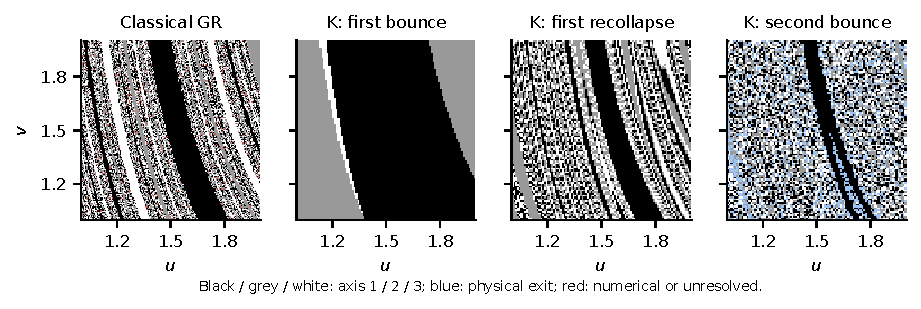
\includegraphics[width=\textwidth]{figs/fig1_basins.pdf}
\caption{Classical reference map (left, $200^2$ points) and corrected finite-event K maps at
$\Lam=20$ ($100^2$ points). Classical labels use the first-$u>7$ outcome; LQC labels identify the
smallest axis at the indicated event. Blue indicates a physical exit before the event; red indicates a numerical
failure or unresolved event. An outcome is retained only if the path up to that event passes the
minimal cutoff. Later failures do not retrospectively remove earlier valid events.}\label{fig:basins}
\end{figure}
\begin{figure}[t]
\centering
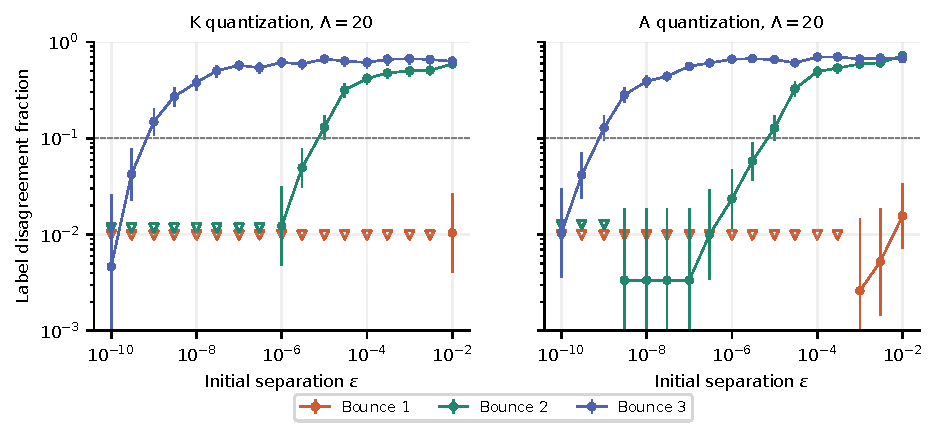
\includegraphics[width=\textwidth]{figs/fig2_uncertainty.pdf}
\caption{Label disagreement at the first three bounces, with 95\% Wilson intervals. Open downward
triangles denote the upper bounds when zero disagreements are observed; their vertical coordinates
are not measured nonzero fractions. Each radius has its own recorded valid-pair denominator.
The dashed line marks $f=0.1$.}\label{fig:uncertainty}
\end{figure}
Figures~\ref{fig:basins} and \ref{fig:uncertainty} describe outcome sensitivity at individual numbered events.
The increasingly interleaved labels motivate a quantitative measure of this refinement, but do not establish a
noninteger asymptotic boundary dimension in LQC. A finite sample with no label changes at a small
radius supplies an upper bound on the disagreement probability. We therefore do not extrapolate a
finite-cycle crossover to infinitely fine structure.

\begin{table}[t]
\caption{Sampled brackets for the level $f=0.1$ and label changes in the tighter-tolerance control. Unbracketed levels are not assigned an artificial smoothing scale.}\label{tab:labels}
\centering
\begin{tabular}{lllr}
\hline
model & event & bracket in $\varepsilon$ & noise flips/pairs\\\hline
\tabrows{label_rows}
\hline
\end{tabular}
\end{table}
Table~\ref{tab:labels} gives the sampled crossover brackets. They describe finite-event sensitivity and the precision of the sampled grid, not uncertainty intervals for an asymptotic exponent.
Nonzero label changes in the tighter-tolerance control limit the interpretation of small measured
fractions at late events. Conversely, the absence of observed control flips only bounds their probability;
it does not certify every label at arbitrarily small perturbations.

\subsection{Amplification over a resolved cycle}
\begin{table}[t]
\caption{Corrected phase and total gains from $R_1$ to $R_2$, in decades, using one common cohort.
Counts are resolved/eligible pairs; brackets are 95\% bootstrap confidence intervals of the median.
The total is the median of the per-pair total, not a sum of phase medians.}\label{tab:phases}
\centering
\begin{tabular}{lrrrr}
\hline
model & $\Lam$ & pairs & bounce window & complete cycle\\\hline
\tabrows{phase_rows}
\hline
\end{tabular}
\end{table}
\begin{figure}[t]
\centering
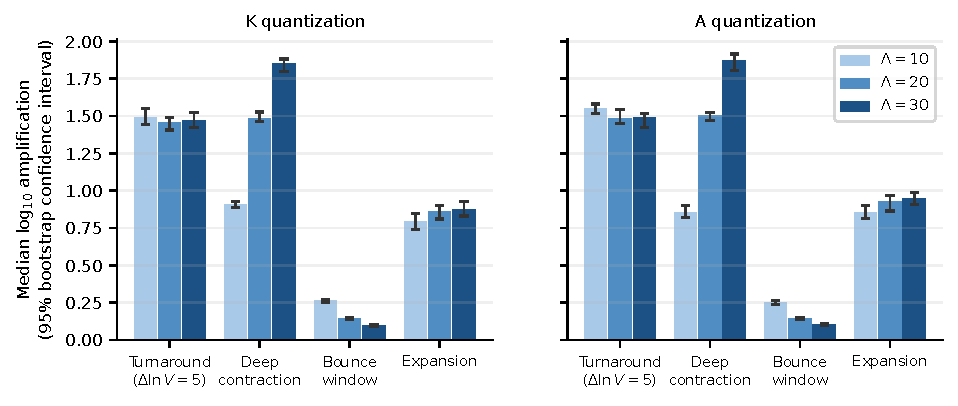
\includegraphics[width=\textwidth]{figs/fig3_phases.pdf}
\caption{Phase gains for the same complete recollapse cycle and cohort as table~\ref{tab:phases}.
Phases are ordered from $R_1$ to $R_2$. The marginal phase medians need not add to the median total.
Whiskers show 95\% bootstrap intervals of medians, not the scatter of individual trajectories.
The turnaround window is five volume e-folds, or $5/3$ mean-scale-factor e-folds.}\label{fig:phases}
\end{figure}
At $\Lam=20$ the measured bounce-window gains are $\KBounce$ (K) and $\ABounce$ (A) decades,
compared with $\KCycle$ and $\ACycle$ for the full cycle (table~\ref{tab:phases}).
Figure~\ref{fig:phases} shows the individual phase gains for the same cohort.
The phase decomposition quantifies amplification outside the selected bounce window,
including the turnaround and subsequent contraction. A large amplification per unit of contraction near recollapse does not imply that most of the total is generated in a fixed five-e-fold window. The relative contributions depend on depth and on the chosen partition.

\begin{figure}[t]
\centering
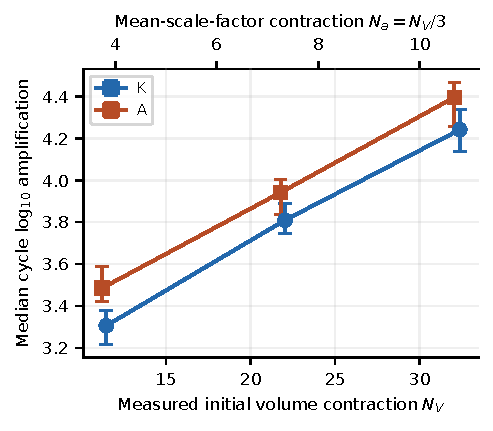
\includegraphics[width=0.6\textwidth]{figs/fig4_rate_vs_depth.pdf}
\caption{Median per-pair full-cycle gain versus measured median initial volume contraction,
using the same resolved cohort for both summaries. The upper axis uses mean-scale-factor e-folds,
differing by a factor of three. Both sets of bars are marginal 95\% bootstrap intervals.}\label{fig:depth}
\end{figure}
Figure~\ref{fig:depth} compares initial scales without identifying $\Lam$ with an exact contraction
depth. Differences between the K and A medians should be interpreted in light of their sampling intervals and their different retained populations. Similar finite-time gains do not establish a universal rate.

\subsection{Cutoff sensitivity, thresholds, and attrition}
\begin{table}[t]
\caption{Sensitivity to the minimum directional length over the entire preceding trajectory,
at $\Lam=20$. The entry 1 is the minimal exclusion criterion, not a sufficient validity theorem.
Counts and intervals have the same meaning as table~\ref{tab:phases}.}\label{tab:cutoff}
\centering
\begin{tabular}{lrrrr}
\hline
model & cutoff / $\ell_{\rm Pl}$ & pairs & bounce window & complete cycle\\\hline
\tabrows{cutoff_rows}
\hline
\end{tabular}
\end{table}
\begin{table}[t]
\caption{Base trajectories reaching each recollapse before any physical or numerical exit,
out of 1000 attempted points per row. Later exits do not invalidate an earlier event.}\label{tab:survival}
\centering
\begin{tabular}{lrrrr}
\hline
model & $\Lam$ & $R_1$ & $R_2$ & $R_3$\\\hline
\tabrows{survival_rows}
\hline
\end{tabular}
\end{table}
\begin{table}[t]
\caption{First stop reason for the three-cycle phase runs (1000 base trajectories each), including the attempted segment $R_3\to P_3$. Physical crossings, constraint failures, and budget exhaustion are distinct.}\label{tab:exits}
\centering
\begin{tabular}{lrrrrrr}
\hline
model & $\Lam$ & complete & physical & constraint & budget & other\\\hline
\tabrows{exit_rows}
\hline
\end{tabular}
\end{table}
Table~\ref{tab:exits} separates the first-exit reasons.
Table~\ref{tab:cutoff} tests whether the result depends on admitting axes only slightly above the
Planck length. These are nested conditional populations; their medians need not coincide.
The contrast between several decades of full-cycle gain and a small bounce-window gain persists
under the $10\ell_{\rm Pl}$ cut. This robustness concerns the retained effective trajectories,
not the validity of a sharply peaked quantum description for every such trajectory.
Table~\ref{tab:survival} reports event survival without combining failed integrations with physical
threshold crossings. The accompanying data list the first physical exits, constraint failures, exhausted
budgets, and other failures separately. Because of attrition, the retained ensemble cannot be identified with a generic late-time invariant measure.

\begin{table}[t]
\caption{Phase-marker variation at $\Lam=20$. From the first 200 base points, one common
cohort passes the validity and numerical controls at all endpoints for all three thresholds.
Counts are identical within each model; this comparison holds the sampled points fixed.}\label{tab:threshold}
\centering
\begin{tabular}{lrrrr}
\hline
model & $h_0$ & resolved pairs & bounce window & complete cycle\\\hline
\tabrows{threshold_rows}
\hline
\end{tabular}
\end{table}
The threshold comparison in table~\ref{tab:threshold} makes the conventional nature of the
bounce-window gain explicit. It does not establish an exact boundary between classical and quantum
evolution. Any statement that the bounce is neutral should therefore be read as a statement about the chosen observables, resolved pairs, and phase markers, rather than about all perturbation directions in the full state space.

\subsection{Six-cycle sensitivity}
\begin{figure}[t]
\centering
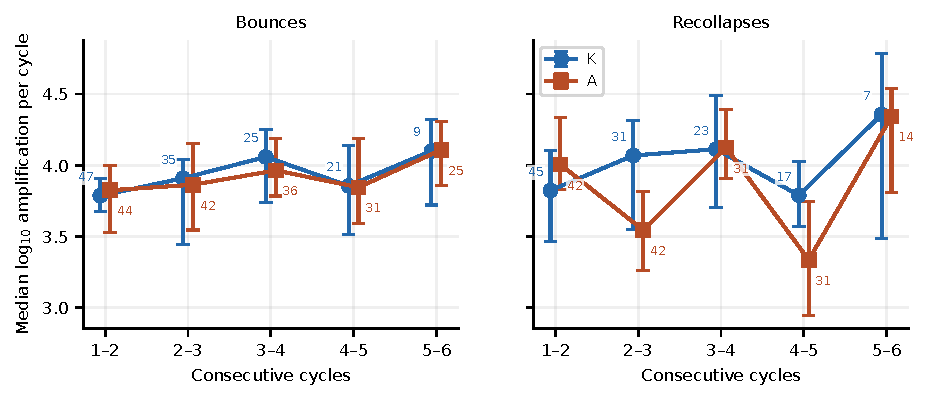
\includegraphics[width=\textwidth]{figs/fig5_longrun.pdf}
\caption{Successive-cycle gains in extended precision at the minimal directional-length cut,
with 95\% bootstrap intervals. Numbers next
to points are resolved pair counts for that step. Different steps can have different retained cohorts;
table~\ref{tab:long} separately uses a fixed cohort across all six cycles.}\label{fig:long}
\end{figure}
\begin{table}[t]
\caption{Mean gain per cycle from event 1 to event 6, calculated for each pair and then summarized
over a fixed cohort resolved at all six events. B and R denote bounce and recollapse sampling.
The length cutoff applies along the entire preceding trajectory; counts are resolved/eligible.
An interval is not estimated for a single pair (CI n/a); small-cohort intervals require particular caution.}\label{tab:long}
\centering
\begin{tabular}{llrrr}
\hline
model & event & cutoff / $\ell_{\rm Pl}$ & pairs & decades/cycle\\\hline
\tabrows{long_rows}
\hline
\end{tabular}
\end{table}
\begin{table}[t]
\caption{Base trajectories reaching each recollapse in the extended-precision experiment, out of
64 attempted points per model, before any physical or numerical exit. The last five columns
separate completion from the first physical or numerical stop reason.}\label{tab:longsurvival}
\centering
\small
\begin{tabular}{lrrrrrrrrrrr}
\hline
model & $R_1$ & $R_2$ & $R_3$ & $R_4$ & $R_5$ & $R_6$ & complete & physical & constraint & budget & other\\\hline
\tabrows{long_survival_rows}
\hline
\end{tabular}
\end{table}
The high-precision analysis uses two perturbation sizes and retains their high and low components
at every cycle. It therefore involves neither a change of storage precision nor a loss of the small initial separations. Figure~\ref{fig:long} and table~\ref{tab:long} test persistence of finite-cycle growth;
neither a small surviving cohort nor approximately similar increments proves an asymptotic limit.
Table~\ref{tab:longsurvival} makes the accompanying attrition explicit. Rejected quality-control
pairs and first-exit counts remain part of the result; unobserved trajectories are not assumed
to behave like the survivors.
The nested cutoffs in table~\ref{tab:long} also quantify how requiring a larger separation from
the Planck length affects the already limited late-cycle cohorts.

For the K quantization, only 9 of the 64 base trajectories complete all six cycles: 53 encounter
the directional-length boundary and 2 exhaust an integration budget. The fixed resolved cohorts
contain 8 bounce-sampled pairs and 7 recollapse-sampled pairs, with median per-cycle gains of
$\KLongB$ and $\KLongR$ decades, respectively. The $3\ell_{\rm Pl}$ cut leaves only one resolved
pair for each event type, and the $10\ell_{\rm Pl}$ cut leaves none. Thus the six-cycle K experiment
cannot establish persistence well away from the length boundary. This limitation is distinct from
the cutoff robustness of the first complete recollapse cycle in table~\ref{tab:cutoff}.
For the A quantization, 29 base trajectories complete six cycles, 30 reach the length boundary, and
5 exhaust the integration budget. At the minimal cut, 25 bounce-sampled and 14 recollapse-sampled
pairs remain resolved at every respective event; their median per-cycle gains are $\ALongB$ and
$\ALongR$ decades. Requiring all directional lengths to exceed $10\ell_{\rm Pl}$ reduces these
cohorts to 5 and 2 pairs. Positive gains persist in these particular survivors, but such small
cohorts do not support a precise ensemble comparison or a general late-cycle rate. Their bootstrap
intervals reflect only resampling of the retained points and cannot account for the missing population.

\section{Discussion and conclusions}
The corrected analysis measures strong finite-cycle sensitivity in the two specified effective
Hamiltonian models, with much smaller scale-factor amplification across the marker-defined bounce
window than over a full recollapse cycle. This quantifies the earlier numerical observation reported in reference~\cite{BlackmoreWilsonEwing2023}. The event construction eliminates the dependence on an arbitrary integration clock, but not on the coordinate and norm choices underlying finite-time separations. The label maps provide complementary outcome sensitivity, not an independently
established fractal dimension of an asymptotic LQC boundary.

Three limitations are central. First, physical and numerical attrition condition every ensemble;
the effective state need not remain sharply peaked even above the directional-length cutoff.
Second, projected separations do not determine information transfer in the complete phase space
or a quantum state. Third, a finite number of cycles cannot settle an infinite-cycle chaos or
mixing question. A return-map study with tangent dynamics, suitable invariant-set evidence, and
controlled treatment of escape from the valid regime would be needed for a stronger conclusion.

Our equations omit inverse-triad corrections~\cite{CorichiKarami2016} and do not test the same
model as the early inverse-volume suppression arguments. We therefore make no general claim about whether quantum gravity creates or removes chaos. Matter, inhomogeneity, and quantum fluctuations
can change the dynamics. Applications to black-hole interiors would require a separate model and
cannot be inferred from recollapse measurements in this closed homogeneous cosmology.

% CONFIRM the funding statement before submission.
\funding{This research received no specific grant from any funding agency in the public, commercial, or not-for-profit sectors.}

\roles{Muhammad Ramadhan: conceptualization, methodology, software, formal analysis, investigation, validation, visualization, writing (original draft), and writing (review and editing).}

\section*{Conflict of interest}
The author declares no competing interests.

\section*{Ethics statement}
This study is purely theoretical and computational and did not involve human participants, human data or tissue, or animals; ethical approval was therefore not required.

\data{The accompanying code-and-data package contains the equations, pinned numerical environments,
raw trajectory records, deterministic seeds, controls, and scripts generating the tables and figures.
The revised results are in \texttt{results/revised/}; the reproduction instructions distinguish them
from the earlier exploratory outputs. A public repository and archival identifier have not yet been
assigned to this revised package.}

\FloatBarrier
\appendix
\section{Explicit evolution equations and verification}\label{app:checks}
Let $c=\gamma^2\Delta/4$ and, for cyclic $(i,j,k)$, define
\begin{align}
E_i&=e^{x_j+x_k-3x_i}, & e_i&=e^{x_i-x_j-x_k},\\
W&=c\left(\sum_i E_i-2\sum_i e_i\right),\\
F_i&=c(-2E_i+2E_j+2E_k-4e_i).
\end{align}
These specify equation~\eqref{eq:eom}. For the A quantization we set
$\psi_i=\theta_i+\phi_i$, $s_i=\sin\psi_i$,
$S_A=\sum_{i<j}s_i s_j$, $c_A=(1+\gamma^2)/\gamma^2$, and
$\eta_i=\sqrt\Delta e^{(x_j+x_k-3x_i)/2}$. The equations are
\begin{align}
x_i'&=\cos\psi_i(s_j+s_k+\eta_i),\\
\theta_i'&=-S_A+\tfrac12\sum_{l\ne i}x_l'(\theta_l-\theta_i)
 -\sum_l x_l'\partial_{x_i}\phi_l-\sum_l\omega_{li}\eta_l s_l+c_A F_i,
\end{align}
where $\omega_{ii}=-1/2$ and $\omega_{li}=3/2$ for $l\ne i$.
The constraint is $S_A+\sum_l\eta_l s_l=c_AW$. With our constant lapse, the physical directional rates are
$H_i=(\sum_jx_j'/2-x_i')/(\gamma\sqrt\Delta)$.

The verification scripts check the Bianchi IX curvature directly in Euler coordinates, the Arnowitt--Deser--Misner (ADM)
Hamiltonian, the classical limits, canonical shifts, and the transformed Hamilton equations.
The A implementation is compared with numerical derivatives of the connection Hamiltonian, and
the classical Bianchi II transition and LQC Bianchi I bounce rules are reproduced. These checks
establish algebraic and numerical consistency of the implemented models; they do not establish
their physical applicability at every state or the statistical interpretation of a finite trajectory.

\section{Numerical controls and reproducibility}
The integrator is a ninth-order Verner method with relative tolerance $10^{-12}$ for the phase and
label runs and $10^{-28}$ for the extended-precision run. The absolute tolerances of the angles scale with their instantaneous magnitudes. Angles are rewrapped using their exact integer and residual representation.
The onset search is staged through small marker thresholds, restarting its clock at each stage.
This avoids loss of event-time resolution after a long preceding contraction. The root-based
length guards use 20 interpolation checks per step, supplemented by accepted-step and endpoint
monitoring. As with any numerical event search, resolution is finite; the regression counterexample
is checked at two tolerances, and the statistical analysis includes independent tighter-tolerance controls.
The extended-precision runs memoize the immutable Verner coefficient tables. Their values are checked
byte for byte against the original constructors; complete controlled trajectory records were also
verified to match exactly. This affects only the execution cost, not the integration algorithm or the accuracy settings.

The normalized constraint residual is $|S-W|/(\sum_i\sin^2\theta_i+c\sum_i(E_i+2e_i))$ for the
K quantization, and the analogous ratio with $s_i=\sin\psi_i$, the terms $|\eta_i s_i|$ and the factor
$c_A$ for the A quantization. The kinetic part is normalized by $\sum_i\sin^2\theta_i\ge|S|$, which
vanishes only if all three sines vanish. Normalizing instead by $\sum_{i<j}|\sin\theta_i\sin\theta_j|$
fails at bounces where two sines pass through zero together: the denominator then collapses and
absolute residuals $\sim10^{-11}$ appear as relative errors of order unity. An earlier version of our
analysis used that normalization and terminated healthy trajectories; re-integrating a sample of them
with the present definition gave no genuine constraint failure. A residual of $10^{-3}$ terminates the
run; it is not an accuracy certificate for trajectory separations. Every event search has a budget of 300000 steps.
Exhaustion of this budget is recorded as an unresolved integration, not as a physical exit. Perturbation and noise checks are made
per pair at the events entering each statistic. Each trajectory has a cumulative cutoff mask;
the mask follows all intermediate integrations, not only the volume extrema.

\begin{table}[t]
\caption{Sensitivity to numerical quality selection at $\Lam=20$ and the minimal length cut.
Strict, primary, and relaxed selections require signal/noise at least 1000, 100, and 10,
respectively, and relative vector discrepancies at most 0.05, 0.1, and 0.2.
All retain the separation bound 0.1. The primary selection defines the headline results.}
\label{tab:quality}
\centering
\begin{tabular}{llrrr}
\hline
model & selection & resolved pairs & bounce window & complete cycle\\\hline
\tabrows{quality_rows}
\hline
\end{tabular}
\end{table}
Table~\ref{tab:quality} shows that tightening the numerical controls substantially reduces the
sample. The full-cycle medians remain several decades, while the bounce-window medians remain
small. The shifts between these conditional populations are an additional selection sensitivity,
not part of the bootstrap sampling intervals.

Files record every point, role, perturbation size, event, cutoff mask, stop reason, and code hash.
The displayed initial-coordinate columns are Float64 summaries; exact extended-precision initial
data are regenerated from the saved point ID and deterministic sampling rule.
Resumption refuses mismatched source or parameter metadata. All revised production files use one
schema, and the analysis refuses to generate manuscript artifacts until the declared runs are complete.
The earlier mixed-precision six-cycle output is retained as historical data and is not used in the
revised tables. Regression tests check that the previously missed sub-Planckian trajectory now
terminates at the crossing, that a trajectory formerly stopped by the collapsing residual
normalization completes its cycle with residual below $10^{-6}$ while a genuine constraint violation
is still detected, and that the median total is distinguished from the sum of medians.

\FloatBarrier
\bibliographystyle{iopart-num-doi}
\bibliography{references}
\end{document}
